\section{JPEG}

\begin{frame}[allowframebreaks]
  \frametitle{Compressão JPEG}
  O padrão JPEG (\textit{Joint Photographers Expert Group}) é amplamente difundido e
  utilizando em câmeras digitais e na internet.

  \vspace{0.5cm}
  Esforço conjunto: ISO/IEC JTC 1 + ITU-T

  International Organization for Standardization (ISO), 
  International Electrotechnical Commission (IEC),
  International Telecommunication Union (ITU)

  \vspace{2ex}
  Ele utiliza a transformada discreta em cossenos (DCT).

  \framebreak
  O padrão é dividido em 6 partes: 
  \begin{enumerate}
  \item Requisitos e diretrizes, %Requirements and guidelines, 
  \item Teste de conformidade, %Compliance testing, Extensions, 
  \item Extensões,
  \item Métodos para registrar parâmetros usados pelo JPEG estendido,
  \item Formato de intercâmbio de arquivos JPEG (JFIF),
  \item Aplicações para sistemas de impressão.
  \end{enumerate}

  \url{https://en.wikipedia.org/wiki/JPEG}

  \framebreak

  \begin{itemize}
  \item método de compressão com/sem perdas (\textit{lossy/lossless}) para imagens coloridas/tons de cinza
  \item não lida bem com imagens de dois níveis (preto e branco)
  \item melhor desempenho em imagens de tom contínuo, onde pixels adjacentes possuem cores similares
  \item utiliza diversos parâmetros que podem ser ajustados 
  \item degradação quase imperceptível de qualidade mesmo para fatores de compressão de 10 a 20
  \end{itemize}

  \framebreak
 
  \begin{figure}[h!]
  \centering
  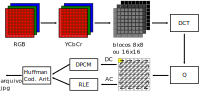
\includegraphics[width=0.8\textwidth]{images/jpegstd.pdf}
  \caption{Esquema do padrão de compressão JPEG.}
  \label{fig:jpegschema}
  \end{figure}

  \framebreak

  A compressão JPEG segue os seguintes passos:
  \begin{enumerate}
  \item Separação em intensidade e cor (RGB - YCbCr). Subdivisão em blocos $8 \times 8$-pixels.
  \item Aplica-se a DCT a cada bloco, armazenados temporariamente com 12 bits (11 bits de precisão e 1 bit de sinal).
  \item Quantização dos blocos de 64 coeficientes através da divisão por uma matriz fixa com
        menor precisão nos termos de alta frequência.
  \item O primeiro coeficiente fornece o brilho médio (DC), sendo codificado pela diferença em relação
        ao mesmo termo no bloco antecessor. 
  \item Os demais 63 coeficientes são organizados em zigzag de baixas frequências até alta frequência
        e são codificados por RLE.
  \item O fluxo de dados final é codificado por código de Huffman ou codificação aritmética.
  \end{enumerate}

  % /home/leoca/ee/ufsj/2012_01/audio_video/aulas/images/dct_basis_func.jpg
  % /home/leoca/ee/ufsj/2012_01/audio_video/aulas/images/take_DCT.png

  \framebreak

  \begin{itemize}
  \item Compressão e descompressão para DCT são simétricos (mesma complexidade computacional e tempo de execução)
  \item Perda de termos de alta frequência acarreta distorções.
  \item Em geral, qualquer compressão com perdas não devem ser utilizadas em imagens destinadas a medições e análise.
  \item Usualmente a análise de qualidade por humanos é empregada para comparar diferentes métodos.
  \end{itemize}

  \framebreak

  \begin{figure}[h!]
  \centering
  \includegraphics[width=0.8\textwidth]{images/jpeg_artifacts.jpg}
  \caption{Artefatos criados pela compressão.}
  \label{fig:jpeg_artifacts}
  \end{figure}


\end{frame}
\note{
Especificação original do JPEG é de 1992.

A compressão de imagens com perdas baseada na DCT foi originalmente proposta por
Nasir Ahmed em 1972.
(Ahmed, Nasir; Natarajan, T.; Rao, K. R. (January 1974), 
`Discrete Cosine Transform', IEEE Transactions on Computers, C-23 (1): 90-93, doi:10.1109/T-C.1974.223784)

Inicialmente o padrão JPEG utilizava apenas a codificação de Huffman, como codificação de entropia.
Existe a possibilidade de utilizar alternativamente a codificação aritmética (levando a arquivos de 5 a 7\% menores), 
porém por causa da proteção de patente, a maior parte dos codificadores e decodificadores implementaram
apenas a codificação de Huffman.
}

\subsection{Subamostragem de Crominância}
\begin{frame}[allowframebreaks]
  \frametitle{Subamostragem de Crominância}
  Notação \textbf{J:a:b}.

  Cada bloco terá $J$ pixels de largura e 2 de altura.

  $a$: número de amostras de crominância presentes na primeira linha \\
  $b$: número de amostras de crominância presentes na segunda linha

  $H$: resolução relativa na direção horizontal\\
  $V$: resolução relativa na direção vertical\\
  $T$: resolução relativa final

  \framebreak

  \begin{figure}[h!]
  \centering
  \includegraphics[width=0.5\textwidth]{images/chromasubsamplefig01.pdf}
  \caption{Esquema de subamostragem de crominância \citep{kerr2012}.}
  \label{fig:chromasubsamplefig01}
  \end{figure}

  \framebreak

  \begin{figure}[h!]
  \centering
  \includegraphics[width=0.5\textwidth]{images/chromasubsamplefig02.pdf}
  \caption{Esquema de subamostragem de crominância \citep{kerr2012}.}
  \label{fig:chromasubsamplefig02}
  \end{figure}

  \framebreak

  \begin{figure}[h!]
  \centering
  \includegraphics[width=0.5\textwidth]{images/chromasubsamplefig03.pdf}
  \caption{Esquema de subamostragem de crominância \citep{kerr2012}.}
  \label{fig:chromasubsamplefig03}
  \end{figure}

\end{frame}
 

\subsection{Quantização dos coeficientes da DCT}
\begin{frame}[allowframebreaks]
  \frametitle{Quantização dos coeficientes da DCT}
  Após o cálculo dos $8 \times 8$ coeficientes da DCT, eles serão quantizados.
  Nesta etapa há efetivamente a perda de informação.

  \vspace{1em}
  Quantização:
  \begin{itemize}
  \item cada coeficiente da DCT é dividido pelo elemento correspondente na tabela de quantização,
  \item o resultado é arredondado para o inteiro mais próximo
  \end{itemize}

  \vspace{2em}
  Cada componente de cor utilizada uma tabela de quantização diferente.
  O padrão JPEG permite a utilização de até quatro tabelas e o usuário pode selecionar
  qualquer uma das quatro para quantizar qualquer componente de cor.

  \framebreak

  As tabelas padrão de quantização. Estas tabelas para luminância e crominância
  são resultado de diversos experimentos realizados pelo comitê do JPEG.

  \vspace{3ex}
  \begin{columns}[c]
  \column{.5\textwidth}
  $
  \begin{bmatrix}
  16 & 11 & 10 & 16 & 24 & 40 & 51 & 61 \\   
  12 & 12 & 14 & 19 & 26 & 58 & 60 & 55 \\  
  14 & 13 & 16 & 24 & 40 & 57 & 69 & 56 \\
  14 & 17 & 22 & 29 & 51 & 87 & 80 & 62 \\
  18 & 22 & 37 & 56 & 68 & 109 & 103 & 77 \\
  24 & 35 & 55 & 64 & 81 & 104 & 113 & 92 \\
  49 & 64 & 78 & 87 & 103 & 121 & 120 & 101 \\
  72 & 92 & 95 & 98 & 112 & 100 & 103 & 99 
  \end{bmatrix}
  $
  luminância
  \column{.5\textwidth}
  $
  \begin{bmatrix}
  17 & 18 & 24 & 47 & 99 & 99 & 99 & 99 \\
  18 & 21 & 26 & 66 & 99 & 99 & 99 & 99 \\
  24 & 26 & 56 & 99 & 99 & 99 & 99 & 99 \\
  47 & 66 & 99 & 99 & 99 & 99 & 99 & 99 \\
  99 & 99 & 99 & 99 & 99 & 99 & 99 & 99 \\
  99 & 99 & 99 & 99 & 99 & 99 & 99 & 99 \\
  99 & 99 & 99 & 99 & 99 & 99 & 99 & 99 \\
  99 & 99 & 99 & 99 & 99 & 99 & 99 & 99 
  \end{bmatrix}
  $
  crominância
  \end{columns}

  \framebreak

  Tabela de quantização simples $Q$ calculada com base em um parâmetro, $R$, definido pelo usuário.
  Os elementos da matriz são dados por $Q_{ij} = 1 + (i + j) \times R$.

  \vspace{3ex}
  Para $R=2$ teremos a seguinte matriz:

  $  
 \begin{bmatrix}
  1 & 3 & 5 & 7 & 9 & 11 & 13 & 15 \\
  3 & 5 & 7 & 9 & 11 & 13 & 15 & 17 \\
  5 & 7 & 9 & 11 & 13 & 15 & 17 & 19 \\
  7 & 9 & 11 & 13 & 15 & 17 & 19 & 21 \\
  9 & 11 & 13 & 15 & 17 & 19 & 21 & 23 \\
  11 & 13 & 15 & 17 & 19 & 21 & 23 & 25 \\
  13 & 15 & 17 & 19 & 21 & 23 & 25 & 27 \\
  15 & 17 & 19 & 21 & 23 & 25 & 27 & 29 
  \end{bmatrix}
  $
  
\end{frame}




\subsection{Imagens de Teste}

\begin{frame}[allowframebreaks]
\frametitle{Imagens de Teste}
  Testar e comparar diferentes método com relação à eficiência e custo computacional.
  \begin{itemize}
  \item Calgary Corpus
  \item Canterbury Corpus
  \item conjunto de documentos do ITU-T para compressão de fax
  \end{itemize}

  \framebreak
  \begin{figure}[h!]
  \centering
  \includegraphics[width=0.5\textwidth]{images/lena_color.jpg}
  \caption{Lena.}
  \label{fig:lena_color}
  \end{figure}
  \framebreak

  \begin{figure}[h!]
  \centering
  \includegraphics[width=0.5\textwidth]{images/mandril.jpg}
  \caption{Mandril.}
  \label{fig:mandril}
  \end{figure}

  \framebreak

  \begin{figure}[h!]
  \centering
  \includegraphics[width=0.5\textwidth]{images/peppers.jpg}
  \caption{Pepers.}
  \label{fig:pepers}
  \end{figure}

  \framebreak

  \begin{figure}[h!]
  \centering
  \includegraphics[width=0.5\textwidth]{images/boat.jpg}
  \caption{Boat.}
  \label{fig:boat}
  \end{figure}

  \framebreak

  \begin{figure}[h!]
  \centering
  \includegraphics[width=0.5\textwidth]{images/barbara.jpg}
  \caption{Barbara.}
  \label{fig:barbara}
  \end{figure}

\end{frame}


\subsection{Outros Formatos JPEG}
\begin{frame}%[allowframebreaks]
  \frametitle{Lossless JPEG}
  \begin{itemize}
  \item 1993
  \item codificação preditiva - DPCM
        \begin{figure}[h!]
        \centering
        \includegraphics[width=0.2\textwidth]{images/pixelprediction.pdf}
        \caption{Esquema de predição de pixel no JPEG sem perdas (Wikipedia).}
        \label{fig:pixelprediction}
        \end{figure}
  \item codificador de entropia - codificação Huffman coding ou codificação aritmética
  \end{itemize}
\end{frame}

\begin{frame}%[allowframebreaks]
  \frametitle{JPEG2000}
  \begin{itemize}
  \item utiliza wavelets
  \item representação em múltiplas resoluções
  \item quantizador escalar com zona morta para codificar os coeficientes
  \item codificação aritmética binária adaptativa guiada por contexto (MQ coder)
  \item patentes
  \end{itemize}
\end{frame}

\begin{frame}%[allowframebreaks]
  \frametitle{JPEG-LS}
  \begin{itemize}
  \item 2003
  \item padrão de compressão sem (ou quase sem) perdas
  \item algoritmo LOCO-I: predição, modelagem do resíduo e codificação do resíduo baseada em contexto
  \item resíduo segue uma distribuição de Laplace
  \item códigos Golomb são quase ótimos para este tipo de distribuição
  \item mais rápido que o JPEG2000 e melhores resultados que o JPEG original
  \end{itemize}
\end{frame}

\begin{frame}%[allowframebreaks]
  \frametitle{JPEG XT}
  JPEG XT (ISO/IEC 18477)
  \begin{itemize}
  \item 2015
  \item Retro compatível com o padrão JPEG (ISO/IEC 10918-1 e ITU Rec. T.81).
  \item Suporte a maior extensão dinâmica (imagens HDR).
  \item Suporte a camada alfa (transparência).
  \item Informações adicionais são salvas como \textit{metadata} do arquivo no padrão JPEG.
  \end{itemize}
\end{frame}

\begin{frame}[allowframebreaks]
  \frametitle{Guetzli}

  \begin{itemize}
  \item Projeto do Google (2017)
  \item \url{https://github.com/google/guetzli}
  \item Guetzli: Perceptually Guided JPEG Encoder (arXiv:1703.04421v1)
  \item utiliza a implementação \texttt{libjpeg} do grupo independente JPE
  \item utiliza a medida de qualidade \texttt{Butteraugli} (utiliza modelos de percepção de cor e
        mascaramento visual)
  \item loop no processo de codificação para encontrar a `melhor' matriz de quantização e descartar
        coeficientes para melhorar o desempenho do RLE
  \item imagens de alta qualidade com redução de aprox. 35\% no tamanho
  \end{itemize}

  \begin{figure}[h!]
  \centering
  \includegraphics[width=0.3\textwidth]{images/guetzliloop.pdf}
  \caption{Otimização global: matriz de quantização. Otimização local: descarte de certos coeficientes \citep{guetzli}.}
  \label{fig:guetzliloop}
  \end{figure}

  Otimização global:
  \begin{itemize}
  \item a tabela de quantização global é uma vetor de tamanho $192 = 3 \times 64$
  \item realiza-se uma busca em um subconjunto de tabelas de quantização
  \end{itemize}

\end{frame}



\begin{frame}%[allowframebreaks]
  \frametitle{Notebook JPEG - GNU Octave}
  \centering
  \includegraphics[width=0.4\textwidth]{images/qrcode-jupyter-jpeg.pdf}

  \url{https://nbviewer.jupyter.org/github/leolca/notebooks/blob/master/aev/jpeg.ipynb}
\end{frame}


